\documentclass{beamer}

\usetheme{simple}

\usepackage[spanish]{babel}
\usepackage[utf8]{inputenc}
\usepackage{csquotes}
\usepackage{fourier}
\usepackage{url}
\usepackage{hyperref}
\usepackage{graphicx}
\graphicspath{{img/}}
%%% BIBLATEX
\usepackage{biblatex}
%%% BIBLIOGRAPHY
\addbibresource{references.bib}
%paquete para trabajar con código
\usepackage{listings}
%paquete para trabajar con colores y definir propios
\usepackage{color}
\usepackage[scale=2]{ccicons}

\newcommand{\dq}[1]{``#1''}

\definecolor{comment-green}{rgb}{0,0.5,0}
\definecolor{bg-light-gray}{HTML}{E9E9E9}
\definecolor{gopher}{HTML}{D0B698}

%% Golang definition for listings
%% http://github.io/julienc91/lstlistings-golang
%%
\RequirePackage{listings}

\lstdefinelanguage{Golang}%
  {morekeywords=[1]{package,import,func,type,struct,return,defer,panic,%
     recover,select,var,const,iota,},%
   morekeywords=[2]{string,uint,uint8,uint16,uint32,uint64,int,int8,int16,%
     int32,int64,bool,float32,float64,complex64,complex128,byte,rune,uintptr,%
     error,interface},%
   morekeywords=[3]{map,slice,make,new,nil,len,cap,copy,close,true,false,%
     delete,append,real,imag,complex,chan,},%
   morekeywords=[4]{for,break,continue,range,goto,switch,case,fallthrough,if,%
     else,default,},%
   morekeywords=[5]{Println,Printf,Error,Print,},%
   sensitive=true,%
   morecomment=[l]{//},%
   morecomment=[s]{/*}{*/},%
   morestring=[b]',%
   morestring=[b]",%
   morestring=[s]{`}{`},%
   }


\lstdefinestyle{go}{
    language=Golang,
    backgroundcolor=\color{gopher},
    basicstyle=\ttfamily,
  	keywordstyle=\bfseries\color{white},
    stringstyle=\color{blue},
    commentstyle=\color{comment-green}\itshape,
    numberstyle=\color{gray},
    identifierstyle=\color{black},
    rulecolor=\color{gray},
    showstringspaces=false,
    escapeinside={\%*}{*)},
    morekeywords={},
    otherkeywords={},
    breaklines=true,
    frame=trbl, 
    framexleftmargin=25pt,
    numbers=left,
    xleftmargin=\parindent,
    frameround=tttt,
    captionpos=b,
    % re tirado de los pelos, pero es lo que hay
    % sacado de:
    % https://tex.stackexchange.com/questions/24528/having-problems-with-listings-and-utf-8-can-it-be-fixed
    inputencoding=utf8,
    extendedchars=true,
    literate={á}{{\'a}}1 {é}{{\'e}}1 {í}{{\'i}}1 {ó}{{\'o}}1 {ú}{{\'u}}1,
}


\lstset{style=go}
\renewcommand{\baselinestretch}{1.5} 


\title{Paradigmas de Lenguajes y Programación}
\subtitle{Golang}
\author{Luciano Serruya Aloisi}
%\institute{\url{http://github.com/famuvie}}
\date{\today



    \begin{minipage}[l]{0.5\textwidth}
        \begin{flushleft}
            
\includegraphics[scale=0.6]{logoUnpsjb.png}\\ % Include a department/university logo - this will require the graphicx package
            \linespread{4}
            \end{flushleft}
    \end{minipage}
    \begin{minipage}[l]{0.4\textwidth}
        \begin{flushright}
            
\includegraphics[scale=0.2]{go-logo.png}\\ % Include a department/university logo - this will require the graphicx package
            \linespread{4}
        \end{flushright}
    \end{minipage}\\[1cm]
}

\begin{document}

\maketitle

\setwatermark[hoffset=-2cm, voffset=-2cm]{
\includegraphics{go-programming-language.png}}
\begin{frame}{Introducción}
  %\framesubtitle{A beamer theme}

    \begin{itemize}
        \item Robert Griesemer, Rob Pike, y Ken Thompson comenzaron el proyecto en el 2007
        \item Para fines del 2009 fue oficialmente presentado
        \item La principal motivación fue que no había surgido ningún lenguaje para sistemas grandes (\emph{grandes}) en la última década
    \end{itemize}
  
\end{frame}



\setwatermark{}

\begin{frame}{Características}

    \begin{columns}
        \column{.5\textwidth}
            \begin{itemize}
                \item Fuertemente tipado (muy fuerte)
                \item Tipado estático
                \item \emph{Memory-safe} (gracias a su recolector de basura) 
                \item Diseñado para ser seguro y performante
            \end{itemize}

        \column{.5\textwidth}
            \begin{figure}[H]
                \centering
                
\includegraphics[scale=0.2]{gopher3d.png}
                %
\includegraphics[scale=0.2, width=0.8\linewidth]{gopher3d.png}
            \end{figure}
    \end{columns}


\end{frame}



%\setwatermark[hoffset=-3cm,voffset=-2cm]{\fontsize{125pt}{125pt}\selectfont{Simple}}

\begin{frame}
    \begin{figure}[H]
        \centering
        %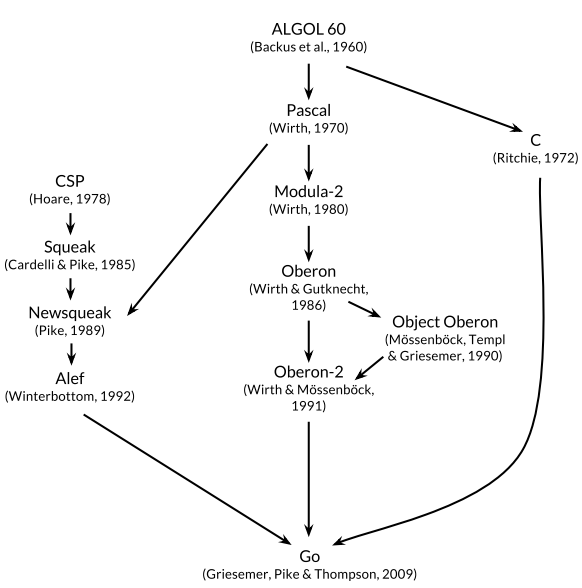
\includegraphics[width=0.8\linewidth, height=8cm]{ancestros.png}
        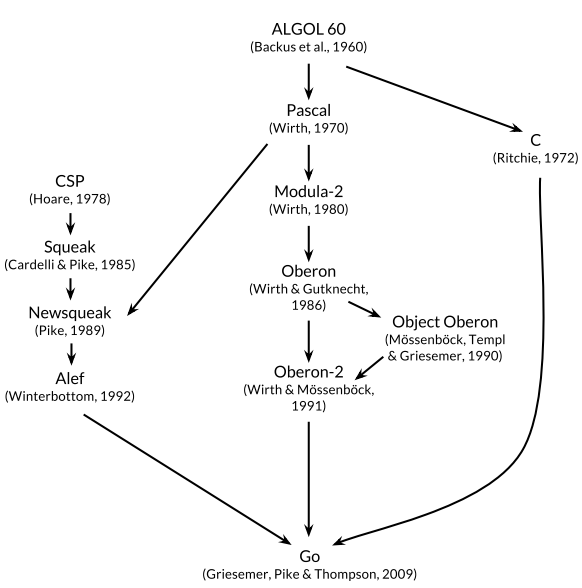
\includegraphics[scale=0.35]{ancestros.png}
        \caption{Ancestros de Go \autocite{BookTheGoProgrammingLanguage:Preface}}
    \end{figure}
\end{frame}


\begin{frame}[fragile]{Demo 1}

{
    \renewcommand{\baselinestretch}{1} 

    \begin{columns}
        \column{.8\textwidth}
        \begin{lstlisting}[title={\dq{Hola mundo!} en Go}]
package main

import "fmt"

func main() {
    fmt.Println("Hello world!")
}
        \end{lstlisting}
    \end{columns}
}
\end{frame}




\setwatermark[hoffset=0.5cm, voffset=-1cm]{
\includegraphics[scale=0.5]{blue-gopher.png}}
\begin{frame}{Estructuras de control}

    \begin{itemize}
        \item \texttt{if..else} 
        \item \texttt{for} 
        \item \texttt{switch} 
    \end{itemize}

\end{frame}

\setwatermark[hoffset=7cm, voffset=-0.2cm]{
\includegraphics[scale=1.2]{aviator-gopher.jpg}}
\begin{frame}{Tipos de datos simples}
    \begin{itemize}
        \item Numéricos
        \begin{itemize}
            \item Enteros
            \item Flotantes
        \end{itemize}
        \item Cadenas
        \item Booleanos
    \end{itemize} 
\end{frame}


\setwatermark{}
\begin{frame}{Tipos de datos complejos}
    \begin{columns}
        \column{.4\textwidth}
        \begin{figure}[H]
            \centering
            
\includegraphics[scale=0.4]{golang.png}
        \end{figure}


        \column{.6\textwidth}
            \begin{itemize}
                \item Arreglos (tamaño fijo)
                \item \emph{Slices} (arreglos con tamaños variantes) 
                \item Mapas
                \item Punteros
                \item \textbf{Registros} 
            \end{itemize}
    \end{columns}
\end{frame}

\begin{frame}[fragile]{Demo 2}

{
    \renewcommand{\baselinestretch}{1} 

    \begin{columns}
        \column{.8\textwidth}
        \begin{lstlisting}[title={Iterando sobre un mapa}]
func imprimeMapa(mapa map[string]int) {
    for k, v := range mapa {
        fmt.Printf("%s: %d\n", k, v)
    }
}
        \end{lstlisting}
    \end{columns}
}
\end{frame}

\begin{frame}{Paradigmas}

    \begin{itemize}
        \item Principalmente \textbf{procedural} 
        \item También permite emular objetos con los \textbf{registros}, \textbf{definición de métodos}, \textbf{registros embebidos}, e \textbf{interfases}   
        \begin{itemize}
            \item Se pueden definir métodos para \emph{casi cualquier tipo de dato} \autocite{TheWayToGo:Methods}, no solamente para aquellos definidos por el usuario 
        \end{itemize}
    \end{itemize}
    
\end{frame}

\begin{frame}[fragile]{Demo 3}

{
    \renewcommand{\baselinestretch}{1} 

    \begin{columns}
        \column{.8\textwidth}
        \begin{lstlisting}[title={Definición de un registro y un método}]
type Persona struct{
    nombre string
    edad int
}
func (pers *Persona) Saludar() string {
    return fmt.Sprtinf("Hola, mi nombre es %s", pers.nombre)
}
        \end{lstlisting}
    \end{columns}
}

\end{frame}

\begin{frame}[fragile]{Demo 4}

{
    \renewcommand{\baselinestretch}{1} 

    \begin{columns}
        \column{.8\textwidth}
        \begin{lstlisting}[title={Interfases y funciones con argumentos variantes}]
type Saludador interface {
    Saludar() string
}

func Saluden(saludadores ...Saludador) {
    for _, obj := range saludadores {
        fmt.Printf("%s\n", obj.Saludar())
    }
}

unaPersona := Persona{"unNombre", 32}
Saluden(&unaPersona)

// "Hola! mi nombre es unNombre"

        \end{lstlisting}
    \end{columns}
}

\end{frame}


\begin{frame}[fragile]{Demo 5}

{
    \renewcommand{\baselinestretch}{1} 

    \begin{columns}
        \column{.8\textwidth}
        \begin{lstlisting}[title={Estructuras complejas mediante composición, no herencia}]
type Alumno struct {
    Persona
    notas []int
}

unAlumno := Alumno{
    Persona{"unNombre", 21},
    int[]{7,8,9},
}

fmt.Printf("%s\n", unAlumno.Saludar())
        \end{lstlisting}
    \end{columns}
}

\end{frame}

\begin{frame}[fragile]{Demo 6}

{
    \renewcommand{\baselinestretch}{1} 

    \begin{columns}
        \column{.8\textwidth}
        \begin{lstlisting}[title={\centering Manejo de situaciones inespereadas a través de devolución de valores de error}]
file, err := os.Open("test.txt")
if err != nil {
    // manejar el error
    return
}
        \end{lstlisting}
    \end{columns}
}

\end{frame}

\begin{frame}[fragile]{\emph{Defer, Panic, Recover}}
    \begin{itemize}
        \item Go no maneja el concepto de \emph{excepciones} 
        \item Dispone de las funciones \texttt{panic} y \texttt{recover}  
        \begin{itemize}
            \item \texttt{panic}: pone el hilo de ejecución en \emph{estado de pánico}  
            \item \texttt{recover}: recupera el control del hilo de ejecución 
        \end{itemize}
        \item Una llamada a \texttt{recover} durante una ejecución normal no tiene ningún efecto 
        \item \texttt{recover} debe estar dentro de una \textbf{función diferida}  
    \end{itemize}
\end{frame}



\begin{frame}[fragile]{Demo 7}

    \begin{itemize}
        \item Las \emph{funciones diferidas} se invocan antes de que termine la ejecución de la función actual
        \item Sirven para cerrar archivos, liberar recursos, y manejar errores
    \end{itemize}
{
    \renewcommand{\baselinestretch}{1} 

    \begin{columns}
        \column{.8\textwidth}
        \begin{lstlisting}[title={Función diferida}]
func main() {
    defer func() {
        fmt.Printf("No' vamoooo'\n")
    }
    fmt.Printf("Algo re importante...\n")
}
// "Algo re importante..."
// "No' vamoooo'"
        \end{lstlisting}
    \end{columns}
}

\end{frame}

\begin{frame}{Concurrencia}
    \begin{columns}
        \column{.4\textwidth}
            \begin{figure}[H]
                \centering
                
\includegraphics[scale=0.25]{notebook-gopher.png}
            \end{figure}
        \column{.6\textwidth}
            \begin{itemize}
                \item Go ejecuta porciones de código de forma concurrente a través de las \texttt{goroutines} 
                \item No necesariamente se corresponde una \texttt{goroutine} con un hilo del SO 
                \item Para comunicarse y sincronizarse varias \texttt{goroutines} se utilizan \textbf{canales} 
                \item Se definen con un tipo de dato, que será el tipo de dato que viajará sobre el canal 
            \end{itemize}
    \end{columns}
\end{frame}

\begin{frame}[fragile]{Demo 8}

{
    \renewcommand{\baselinestretch}{1} 

    \begin{columns}
        \column{.8\textwidth}
        \begin{lstlisting}[title={Ejecución concurrente con \texttt{goroutines} \autocite{GolangBotGoroutines}}]
func hello() {
    fmt.Println("Hello world goroutine")
}
func main(){
    go hello()
    fmt.Println("main function")
}
        \end{lstlisting}
    \end{columns}
}

\end{frame}

\begin{frame}{Canales}
    \begin{itemize}
        \item Las operaciones sobre un canal son \textbf{bloqueantes} 
        \begin{itemize}
            \item Si una \texttt{goroutine} intenta leer (\texttt{<- c}) sobre un canal vacío, se bloqueará hasta que otra \texttt{goroutine} escriba en ese canal 
            \item Si una \texttt{goroutine} intenta escribir (\texttt{c <- }) en un canal que esté lleno (en el caso de los canales con buffer), se bloqueará hasta que otra \texttt{goroutine} lea del canal  
        \end{itemize}
    \end{itemize}
\end{frame}

\begin{frame}{¿Qué pasa con los otros paradigmas?}
    Para implementar otros paradigmas será necesario
    
\end{frame}

\begin{frame}{¿Qué pasa con los otros paradigmas?}
    Para implementar otros paradigmas será necesario
    \begin{columns}
        \column{.5\textwidth}
        \begin{figure}[H]
            \centering
            
\includegraphics[width=0.8\linewidth]{pico.png}
        \end{figure}
        \column{.5\textwidth}
    \end{columns}
\end{frame}

\begin{frame}{¿Qué pasa con los otros paradigmas?}
    Para implementar otros paradigmas será necesario
    \begin{columns}
        \column{.5\textwidth}
        \begin{figure}[H]
            \centering
            
\includegraphics[width=0.8\linewidth]{pico.png}
        \end{figure}
        \column{.5\textwidth}
        \begin{figure}[H]
            \centering
            
\includegraphics[width=0.8\linewidth]{pala.png}
        \end{figure}
    \end{columns}
    
\end{frame}

\begin{frame}{¿Preguntas?}
    \begin{figure}[H]
        \centering
        
\includegraphics[width=0.8\linewidth]{nerd-gopher.png}
    \end{figure}
\end{frame}

\begin{frame}{¡Gracias!}
    \begin{figure}[H]
        \centering
        
\includegraphics[width=0.8\linewidth]{king-gopher.png}
        \caption{}
        \label{fig:}
    \end{figure}
\end{frame}

%%%%%%%%%%%%%%%%%%%%%%%%%%%%%%%%%
% REFERENCIAS
%%%%%%%%%%%%%%%%%%%%%%%%%%%%%%%%%
\begin{frame}{Referencias}
    \printbibliography
\end{frame}

\end{document}
